\documentclass[%
  aspectratio=169,
  9pt,
%   t,
%  USenglish,
ngerman,
%   dark,
  light,
  mathserif,
%   serif, 
  professionalfont,
%  handout,
%  affiliationinhead,
  affiliationintitlepagehead,
  titlegraphic,
  %% The following options would violate the CD rules!
   affiliation,
%   uselogos,
   navigationbar,
  progressbar,
%   seprules,
%   titleinhead,
]{beamer}

\usepackage[utf8]{inputenc}
\usepackage[english, ngerman]{babel}
\usepackage[]{csquotes}

\usepackage{siunitx}

\sisetup{%
	mode = math,
	detect-family,
	detect-weight,  
	exponent-product = \cdot,
	number-unit-separator=\text{\,},
	output-decimal-marker={\text{,}},
	math-rm=\mathsf,
	text-rm=\sffamily,
}

\usepackage{animate}
%\usepackage{MnSymbol,wasysym}

%\newcommand{\org}{LMF}
% \newcommand{\org}{FPF}
%\newcommand{\coorg}{DLR}
\newcommand{\boldstruct}[1]{\textbf{\structure{#1}}}
\usetheme{TUM}
\usepackage{glossaries}
\usepackage{graphicx}
\usepackage{nth}
%\usepackage{natbib}
\usepackage[square,sort,comma,numbers]{natbib}
\bibliographystyle{abbrvnat}
\setcitestyle{authoryear}%,open={((},close={))}

\usepackage{tummath}
\usepackage{tumtensors} % experimental
\usepackage{tumcolors}
\usepackage{subfigure}
\usepackage[noabbrev, capitalize]{cleveref}
\usepackage{csvsimple}
\usepackage{colortbl}
\usepackage{tabularx}
\usepackage{multimedia}

\PassOptionsToPackage{cmyk}{xcolors}
	
\usepackage{booktabs}
\usepackage{contour}

%\usepackage{biblatex}
%\addbibresource{bib/ijgi}

\usepackage{pgfplots}
\usepgfplotslibrary{groupplots}
\usepackage{pgfplotstable}
\usepgfplotslibrary{dateplot}

%\usepgfplotslibrary{external}
%\tikzexternalize

\usepackage{booktabs}
\usepackage{array}
\newcolumntype{x}{l}
\newcolumntype{X}{>{}l}
\newcolumntype{v}[1]{>{\raggedright\hspace{0pt}}p{#1}}
\newcolumntype{V}[1]{>{\scriptsize\raggedright\hspace{0pt}}p{#1}}


\definecolor{fusionremovedcolor}{HTML}{00CA43}
\definecolor{fusionaddedcolor}{HTML}{FF00F7}
\definecolor{overlapcolor}{HTML}{FAC843}

\usepgfplotslibrary{external}
%\tikzexternalize
\tikzsetexternalprefix{tikz/}

%\usetikzlibrary{mindmap}

%\usetikzlibrary{arrows} 
%\usetikzlibrary{backgrounds}
\usetikzlibrary{fit}
%\usetikzlibrary{shapes}
\usetikzlibrary{calc}
\usetikzlibrary{positioning}
\usetikzlibrary{matrix}
\usepackage[nodayofweek,level]{datetime}
%\usepackage{mwe}
%%
%
\usetikzlibrary{3d}
\tikzstyle{perspective3d}=[
x={(0.5cm,0.5cm)}, y={(1cm,0cm)}, z={(0cm,1cm)}]


\colorlet{traincolor}{tumbluelight}
\colorlet{validcolor}{tumbluedark}
\colorlet{evalcolor}{tumorange}

\colorlet{forwardcolor}{tumblue}
\colorlet{backwardcolor}{tumorange}

\colorlet{activationcolor}{tumblue}
\colorlet{gridcolor}{tumgraylight}
\colorlet{contextonecolor}{tumorange}
\colorlet{contexttwocolor}{tumorange!80}
\colorlet{contextthreecolor}{tumorange!60}
\colorlet{contextfourcolor}{tumorange!40}

% defaultvalue -> might be replaced later
\colorlet{tensorcolor}{forwardcolor}

\colorlet{classcolor}{tumivory}
\colorlet{encodercolor}{tumblue}
\colorlet{encodercolor}{tumred}

%\usepackage{media9}

% notation
\newcommand{\MWeight}{\ensuremath{\M{W}}}
\newcommand{\VBias}{\ensuremath{\V{b}}}
\newcommand{\VInput}{\DataVec}
\newcommand{\VHidden}{\ensuremath{\V{h}}}
\newcommand{\FActivation}{\ensuremath{\sigma}}
\newcommand{\VCellState}{\ensuremath{\V{c}}}
\newcommand{\VForgetGate}{\ensuremath{\V{f}}}
\newcommand{\VModulationGate}{\ensuremath{\V{j}}}
\newcommand{\VInputGate}{\ensuremath{\V{i}}}
\newcommand{\VOutputGate}{\ensuremath{\V{o}}}



\newcommand{\VResetGate}{\ensuremath{\V{r}}}
\newcommand{\VUpdateGate}{\ensuremath{\V{u}}}

%\newcommand{\concat}[2]{\VecDef{#1 \Vert #2}}
\newcommand{\concat}[2]{[#1\Vert#2]}

\newcommand{\Rin}[3]{\mathbb{R}^{[#1 \times #2 \times #3]}}
\newcommand{\Rinfloor}[3]{\mathbb{R}^{[#1]} \times \mathbb{R}^{[#2]} \times \mathbb{R}^{[#3]}}
\newcommand{\Rinfour}[4]{\mathbb{R}^{[#1 \times #2 \times #3 \times #4]}}

% kernel size of rnn convolution
\newcommand{\krnn}{k_{rnn}}
% kernel size of classification convolution
\newcommand{\kclass}{k_{class}}

\newcommand{\eg}{e.g., }
\newcommand{\ie}{i.e. }

%\newcommand{\classname}[1]{\texttt{#1}}
\newcommand{\classname}[1]{\textsl{#1}} % what about \textsl for classnames?
\newcommand{\cn}[1]{\classname{#1}} % short alias

\newcommand{\nutzungscn}[1]{\textsc{#1}} % stmelf Nutzungsklassen

\newcommand{\brand}[1]{\textsc{#1}}
\newcommand{\processing}[1]{\brand{#1}}
\newcommand{\satellite}[1]{\brand{#1}}
\newcommand{\band}[1]{\brand{#1}}

% https://tex.stackexchange.com/questions/167925/how-to-make-maths-equations-start-at-the-left
\newcommand{\mathleft}{\@fleqntrue\@mathmargin0pt}
\newcommand{\mathcenter}{\@fleqnfalse}

\usetikzlibrary{spy}

% \usepackage[ngerman]{babel} % if you get errors on compile: rm *aux *out *log *nav *snm *toc

\newcommand{\rastergrid}{
	\input{images/rastergrid.tikz}
}
\newcommand{\vectorgrid}{
	\input{images/vectorgrid.tikz}
}

%\setbeamersize{description width=0mm}

\mode<handout>{
  \usepackage{pgfpages}
% feel free to use one of these layouts
%   \pgfpagesuselayout{1 on 1}[a4paper,border shrink=5mm]
  \pgfpagesuselayout{2 on 1}[a4paper,border shrink=5mm]
%   \pgfpagesuselayout{3 on 1}[a4paper,border shrink=5mm]
%   \pgfpagesuselayout{4 on 1}[a4paper,border shrink=5mm]
%   \pgfpagesuselayout{2 on 1 landscape}[a4paper,border shrink=5mm]
%   
% you can also add room for notes, but then the widescreen aspect ratio messes up a little
%   \usepackage{handoutWithNotes}
%   \pgfpagesuselayout{1 on 1 with notes}[a4paper,border shrink=5mm]
%   \pgfpagesuselayout{2 on 1 with notes}[a4paper,border shrink=5mm]
%   \pgfpagesuselayout{3 on 1 with notes}[a4paper,border shrink=5mm]
%   \pgfpagesuselayout{4 on 1 with notes}[a4paper,border shrink=5mm]
%   \pgfpagesuselayout{1 on 1 with notes landscape}[a4paper,border shrink=5mm]
%   \pgfpagesuselayout{2 on 1 with notes landscape}[a4paper,border shrink=5mm]
}

%% Custom Packages %%%%%%%%%%%%%%%%%%%%%%%%%%%%%%%%%%%%%%%%%%%%%%%%%%%%%%%%%%%%%%%%%%%%
\usepackage{minted}

%%%%%%%%%%%%%%%%%%%%%%%%%%%%%%%%%%%%%%%%%%%%%%%%%%%%%%%%%%%%%%%%%%%%%%%%%%%%%%%%%%%%%%%

%Convolutional-Recurrent Networks for Multi-temporal Classification
\title{Convolutional LSTMs for Cloud-Robust Classification \\ of Remote Sensing Imagery}
%\subtitle{NeurIPS 2018 Workshop on Spatiotemporal Modeling and Decision-making}
\subtitle{$\Phi$-week 2019}
\author[M. Rußwurm, M. Körner]{Marc Rußwurm, Marco Körner}
\institute[TUM]{Technical University of Munich\\Chair of Remote Sensing Technology\\Computer Vision Research Group\\\url{www.lmf.bgu.tum.de/vision}}

\date{13th September 2019, ESA ESRIN, Frascati, Italy}

\begin{document}

\begin{frame}[t]
  \titlepage
\end{frame}

\begin{frame}
\frametitle{When we think of satellite images we picture this}
%\centering\includegraphics[width=.75\textwidth]{images/montreal_satellite}
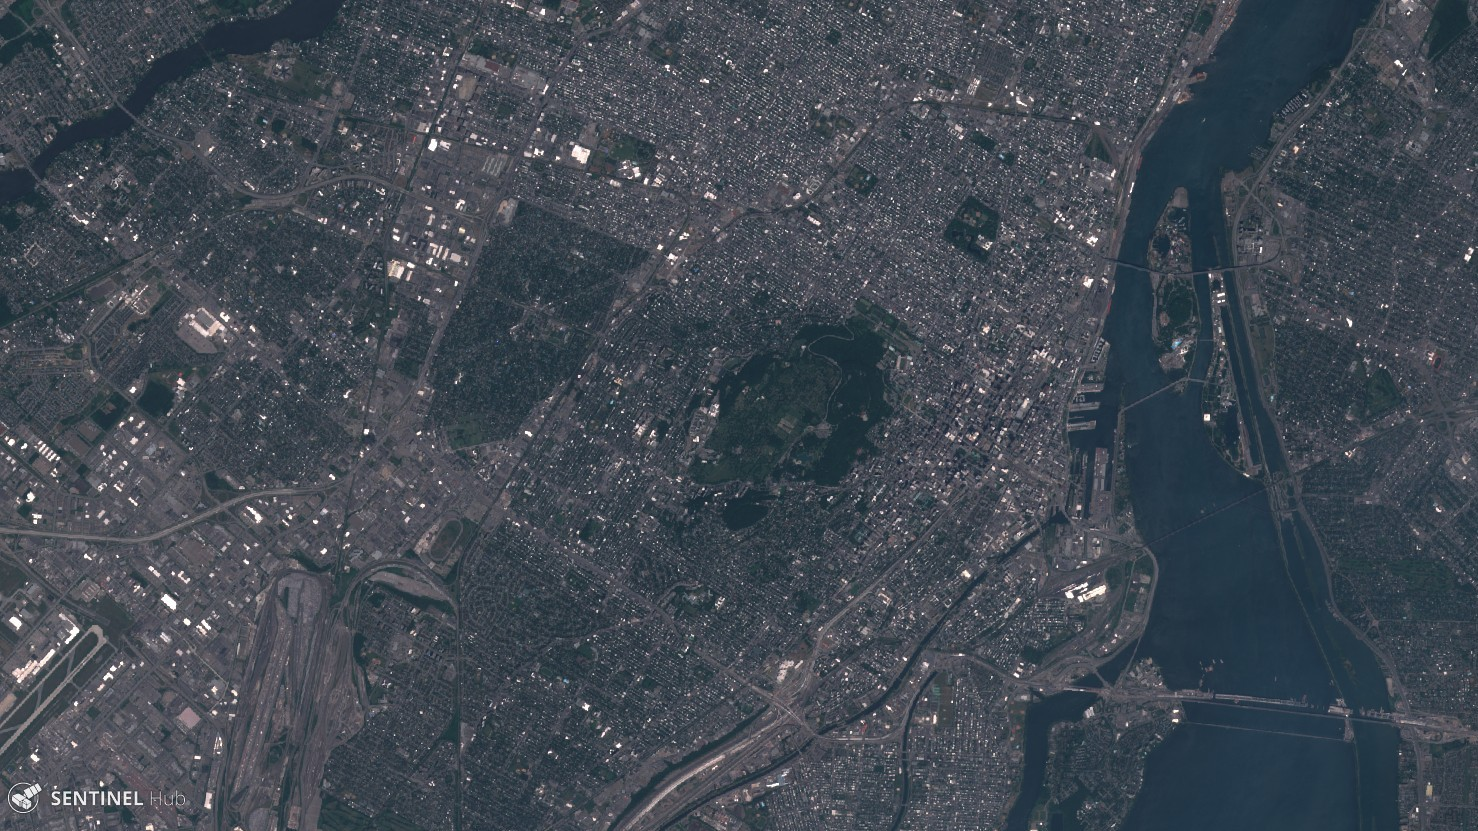
\includegraphics[width=\textwidth]{images/cloudfree}
\end{frame}

\begin{frame}
	\frametitle{... however, ususally }
		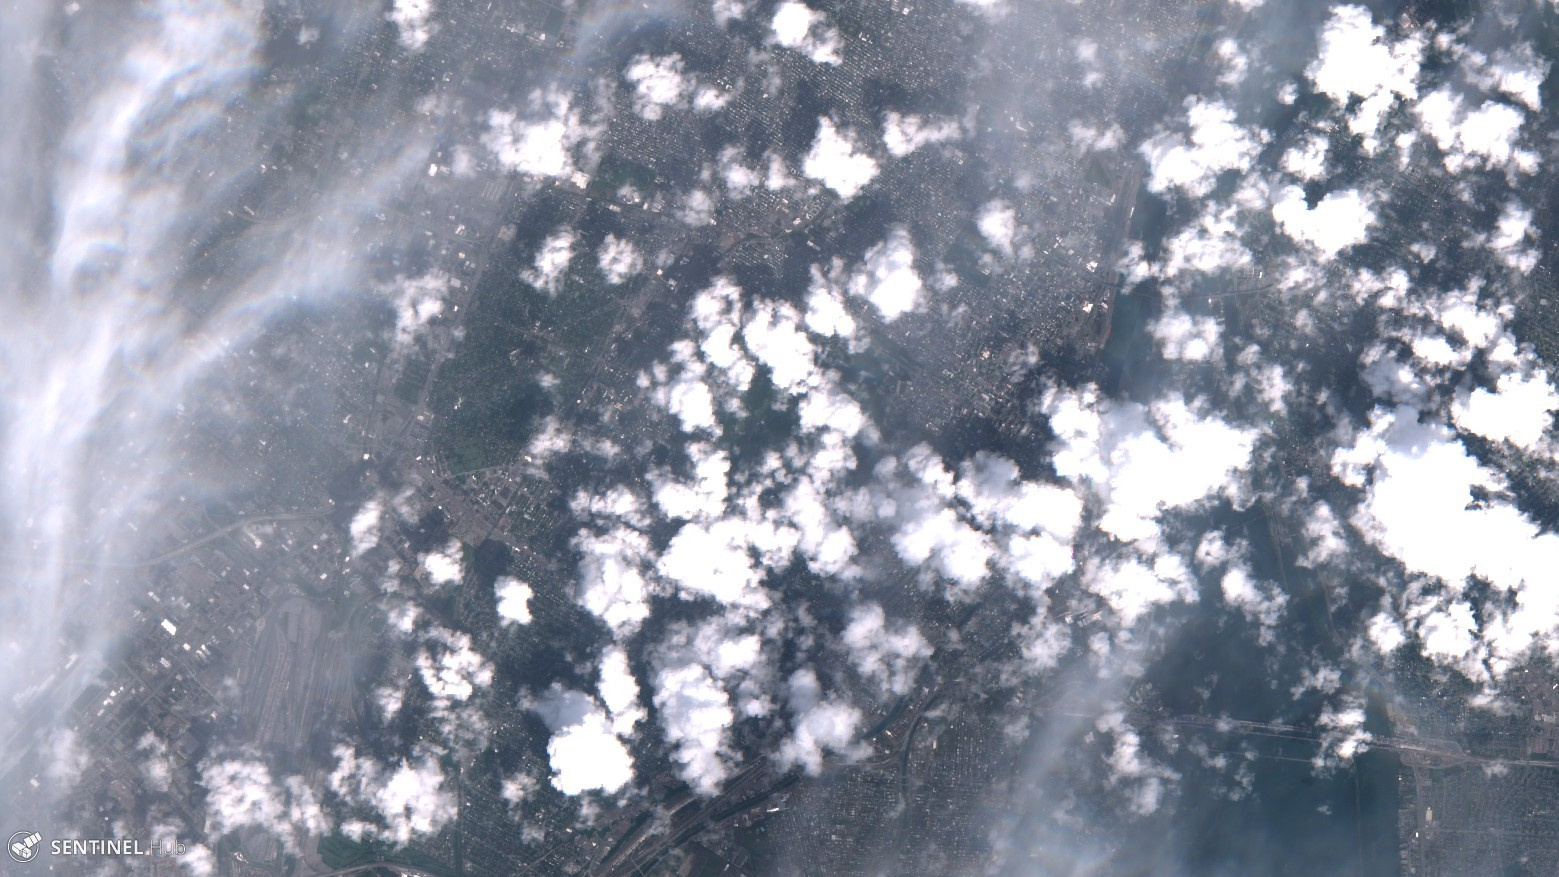
\includegraphics[width=\textwidth]{images/clouds}
	
%		\includegraphics[width=\textwidth]{images/cloud_airplane}
		
\end{frame}

\begin{frame}
	\frametitle{Cloud coverage as spatiotemporal noise}
	\centering
	
	\def\imagewidth{1.5cm}
	
	\includegraphics[width=\imagewidth]{images/activations/16494/x/x-0.png}
	\includegraphics[width=\imagewidth]{images/activations/16494/x/x-1.png}
	\includegraphics[width=\imagewidth]{images/activations/16494/x/x-2.png}
	\includegraphics[width=\imagewidth]{images/activations/16494/x/x-3.png}
	\includegraphics[width=\imagewidth]{images/activations/16494/x/x-4.png}
	\includegraphics[width=\imagewidth]{images/activations/16494/x/x-5.png}
	\includegraphics[width=\imagewidth]{images/activations/16494/x/x-6.png}
	\includegraphics[width=\imagewidth]{images/activations/16494/x/x-7.png}
	\includegraphics[width=\imagewidth]{images/activations/16494/x/x-8.png}
	\includegraphics[width=\imagewidth]{images/activations/16494/x/x-9.png}
	\includegraphics[width=\imagewidth]{images/activations/16494/x/x-10.png}
	\includegraphics[width=\imagewidth]{images/activations/16494/x/x-11.png}
	\includegraphics[width=\imagewidth]{images/activations/16494/x/x-12.png}
	\includegraphics[width=\imagewidth]{images/activations/16494/x/x-13.png}
	\includegraphics[width=\imagewidth]{images/activations/16494/x/x-14.png}
	\includegraphics[width=\imagewidth]{images/activations/16494/x/x-15.png}
	\includegraphics[width=\imagewidth]{images/activations/16494/x/x-16.png}
	\includegraphics[width=\imagewidth]{images/activations/16494/x/x-18.png}
	\includegraphics[width=\imagewidth]{images/activations/16494/x/x-19.png}
	\includegraphics[width=\imagewidth]{images/activations/16494/x/x-20.png}
	\includegraphics[width=\imagewidth]{images/activations/16494/x/x-21.png}
	\includegraphics[width=\imagewidth]{images/activations/16494/x/x-22.png}
	\includegraphics[width=\imagewidth]{images/activations/16494/x/x-23.png}
	\includegraphics[width=\imagewidth]{images/activations/16494/x/x-24.png}
	\includegraphics[width=\imagewidth]{images/activations/16494/x/x-25.png}
	\includegraphics[width=\imagewidth]{images/activations/16494/x/x-26.png}
	\includegraphics[width=\imagewidth]{images/activations/16494/x/x-27.png}
	\includegraphics[width=\imagewidth]{images/activations/16494/x/x-28.png}
	\includegraphics[width=\imagewidth]{images/activations/16494/x/x-29.png}
	\includegraphics[width=\imagewidth]{images/activations/16494/x/x-30.png}
	\includegraphics[width=\imagewidth]{images/activations/16494/x/x-31.png}
	\includegraphics[width=\imagewidth]{images/activations/16494/x/x-32.png}
	\includegraphics[width=\imagewidth]{images/activations/16494/x/x-33.png}
%	\includegraphics[width=\imagewidth]{images/activations/16494/x/x-34.png}
%	\includegraphics[width=\imagewidth]{images/activations/16494/x/x-35.png}
%	
\end{frame}
%
%\begin{frame}
%\LARGE
%\centering
%\textbf{Filter this temporal noise by pre-classificaition?}
%\end{frame}

%\begin{frame}
%		
\usepgfplotslibrary{groupplots}

\tikzsetnextfilename{scl}
\begin{tikzpicture}

%\def\data{images/classhist/classHistograms.dat}
\def\data{images/clouds/scl2.csv}

\pgfplotsset{ every non boxed x axis/.append style={x axis line style=-},
	every non boxed y axis/.append style={y axis line style=-}}

\pgfplotsset{every axis/.append style={ybar=1pt, bar width=6pt, ymajorgrids}}
\pgfplotsset{every axis label/.append style={font=\footnotesize},tick pos=left,ylabel near ticks}
\pgfplotsset{every tick label/.append style={font=\scriptsize}}
%\pgfplotsset{every x tick label/.append style={rotate=90,anchor=east,font=\tiny}}
%   \pgfplotsset{every y tick label/.append style={/pgf/number format/.cd, fixed, precision=2, fixed zerofill,}}
%\tikzstyle{caption}=[font=\footnotesize, fill=tumwhite, fill opacity=.5, text opacity=1]


\begin{axis}[
%group style={
%	%       group size=1 by 4,
%	group size=1 by 1,
%	xlabels at=edge bottom,
%	xticklabels at=edge bottom,
%	ylabels at=edge left,
%	yticklabels at=edge left,
%	vertical sep=2pt,
%	horizontal sep=2pt
%},
width=\textwidth,
height=5cm,
%ymode=log,
%log origin=infty,
%     y dir=reverse,
%     scaled ticks=true,
%log ticks with fixed point,
%scaled x ticks=true,
axis lines=left,
xlabel={image acquisition dates},
ylabel={cloud coverage},
xlabel style={yshift=-2mm},
xmin=-.5,
xmax=46,
%xlabel=clouds,
ytick={1,10,25,50,100},
yticklabels={\SI{1}{\percent},\SI{10}{\percent},\SI{25}{\percent},\SI{50}{\percent},\SI{100}{\percent}},
xtick=data,
xticklabels={
	03. Jan,
	13. Jan,
	20. Jan,
	21. Jan,
	28. Jan,
	12. Feb,
	11. Mär,
	20. Mär,
	23. Mär,
	03. Apr,
	13 Apr.,
	19. Apr,
	22. Apr,
	29. Apr,
	02. Mai,
	10. Mai,
	22. Mai,
	29. Mai,
	08. Jun,
	18. Jun,
	28. Jan,
	02. Jul,
	14. Jul,
	18. Jul,
	21. Jul,
	28. Jul,
	30. Jul,
	07. Aug,
	17. Aug,
	20. Aug,
	28. Aug,
	21. Aug,
	09. Sep.,
	12. Sep..,
	18. Sep.,
	26. Sep.,
	29. Sep.,
	09. Okt.,
	18. Okt.,
	28. Okt.,
	09. Nov.,
	15. Nov.,
	18. Nov.,
	28. Nov.,
	06. Dez.,
	08. Dez.
},
axis on top
];

\addplot[
%       draw=tumblue,
draw=none,
fill=tumblue,rounded corners=.5pt
] table [col sep=comma, x=id, y=cloudpercent] {\data};


\end{axis}
\end{tikzpicture}
%\end{frame}


\input{images/overviewgraphs.tikz}

\begin{frame}<presentation:0>

\frametitle{Detecting Clouds is rarely the main objective}
\LARGE
\centering\figcloudfilteringpipeline

\end{frame}

%


%\begin{frame}<presentation:1>
%
%\frametitle{Introducing a model to pre-classify clouds?}
%\LARGE
%\centering\figcloudfilteringpipeline
%
%\end{frame}

%\begin{frame}
%\frametitle{Clouds classification works very well...}
%
%\includegraphics[width=\textwidth]{images/Li18_clouds}
%
%\texttt{\small Li, Z., Shen, H., Cheng, Q., Liu, Y., You, S., \& He, Z. (2018). Deep learning based cloud detection for remote sensing images by the fusion of multi-scale convolutional features. arXiv preprint arXiv:1810.05801.}
%\end{frame}
%
%\begin{frame}<presentation:2>
%
%\frametitle{Identifying clouds is rarely the main objective!}
%\LARGE
%\centering\figcloudfilteringpipeline
%
%\end{frame}


\begin{frame}
\frametitle{End-to-end trainable model for robust classification}
\LARGE
\centering\figourapproach		

\end{frame}

\begin{frame}
	\frametitle{Gated Recurrence}
	
	
\end{frame}

\newcommand{\attention}{
\begin{tikzpicture}[scale=0.25]
\foreach \t in {1,2,3,4} {
	\node[draw, circle, inner sep=.2em] at (\t, 0){};
}
\end{tikzpicture}
}

\newcommand{\attnv}{
	\begin{tikzpicture}[scale=0.25]
	\foreach \t in {1,2,3,4} {
		\node[draw, circle, inner sep=.2em] at (0, \t){};
	}
	\end{tikzpicture}
}

\newcommand{\attnout}{
	\begin{tikzpicture}[scale=0.25]
	\foreach \t in {1} {
		\node[draw, circle, inner sep=.2em] at (0, \t){};
	}
	\end{tikzpicture}
}

\begin{frame}
	\frametitle{Attention}
	
	\begin{columns}
		\column{.5\textwidth}
		
		
		\attention
		
		\attnv
		
		\begin{tikzpicture}[node distance=.2em]
		\node(alpha){\attention};
		\node[right=of alpha](out){\attnout};
		\node[above=of out]{\attnv};
		\end{tikzpicture}
		
		%	\begin{equation*}
		%		\text{Attention}(Q,K,V) = 
		%		\begin{tikzpicture}
		%		\node(alpha){$\underbrace{\attention}_\alpha$};
		%		\node[right=of alpha](out){};
		%		\node[above=of out]{\attnv};
		%		\end{tikzpicture}
		%		 
		%	\end{equation*}
		
		\Large
		\begin{equation*}
		\text{Attention}(Q,K,V) = \underbrace{\text{softmax}\left(QK^T\right)}_\alpha V
		\end{equation*}
		query: $Q \in \mathbb{R}^{t \times d_k}$
		
		key: $K \in \mathbb{R}^{t \times d_k}$
		
		value: $V \in \mathbb{R}^{t \times d_v}$
		
		attention scores $\alpha \in [0,1]^{t \times t}$
		
		
		\column{.5\textwidth}
		
		
		\begin{tikzpicture}
		\begin{axis}[height=3cm,width=\textwidth,grid=major,]
		\addplot coordinates {(0,.3) (1,.1) (2,.3) (3,.4)};
		\end{axis}
		\end{tikzpicture}
		\begin{tikzpicture}
			
			\begin{axis}[ybar,height=3cm,width=\textwidth,grid=major,]
			\addplot coordinates {(1,.05) (0,.4) (3,.05) (2,.5)};
			\end{axis}
		\end{tikzpicture}
	\end{columns}
	
	\end{frame}


\def\fps{3}
\input{images/cells.tikz}

\begin{frame}[t]
\frametitle{Extracting features from noisy data with ConvRNNs}

\centering
		%\lstmanim
		\begin{tikzpicture}[scale=1, node distance=2em]%,show background rectangle,background rectangle/.style={draw=red}]
		
		
		\draw pic (LSTM) at (0,0) {lstmanim};
		\node[io,xshift=1ex,above=3em of LSTMtl, ,label=above:$\VInput_{t}$](xt){\animategraphics[poster=25,width=1cm,autoplay,loop]{\fps}{images/activations/16494/x/x-}{1}{36}};%$x_{t}$
		\draw[rounded corners] (xt) |- (LSTM-input);
		\node[io,left=of LSTMtl,label=below:$\VHidden_{t-1}$](htminus1){
			\animategraphics[poster=24,width=1cm,autoplay,loop]{\fps}{images/activations/16494/output/3-}{0}{35}
		};
		\draw[endflow] (htminus1) -- (LSTM-input);
		\node[io,right=of LSTMbr,label=above:$\VCellState_{t}$](ct){\animategraphics[poster=25,width=1cm,autoplay,loop]{\fps}{images/activations/16494/state/3-}{1}{36}}; % $c_{t}$
		\draw[endflow] (LSTM-coutput)--(ct);
		\node[io,left=of LSTMbl,label=above:$\VCellState_{t-1}$](ctminus1){\animategraphics[poster=24,width=1cm,autoplay,loop]{\fps}{images/activations/16494/state/3-}{0}{35}}; % 
		\draw[endflow] (ctminus1)--(LSTMfmult);
		\node[io,right=of LSTMtr,label=below:$\VHidden_{t}$](ht){
			\animategraphics[poster=24,width=1cm,autoplay,loop]{\fps}{images/activations/16494/output/3-}{1}{36}
		};
		\draw[endflow] (LSTM-houtput)--(ht);
		
		\draw[endflow] (ct) -- ($ (ct)+(0,-0.8) $) -| (ctminus1);
		\draw[endflow] (ht) -- ($ (ht)+(0,.8) $) -| (htminus1);
		
		\end{tikzpicture}
	
\end{frame}

\begin{frame}<presentation:3>
	\frametitle{Employ ConvRNNs for Vegetation Land Cover Classification directly}
%	\input{images/seqencnetwork.tikz}
%	\figseqencnetwork
	\input{images/network.tikz}
%	
%	\input{images/lstm.tikz}
%	\lstmanimtwo
t\end{frame}

\begin{frame}
\frametitle{It worked very well}
\input{approaches_transposed.tex}
\end{frame}

%
\begin{frame}<presentation:4-5>
\frametitle{Let's look at a few Examples}
\framesubtitle{Sentinel 2 preprocessed by 
\includegraphics[width=4em]{images/GAF_logo}}


\begin{tikzpicture}[baseline=-2em, inner sep=0]

\begin{axis}[
width=\textwidth,
%	hide axis,
height=5.5cm,
ymin=0, ymax=1.2,
%no marks,  
draw opacity=.8,
smooth=0.001,
legend style={at={(.65,1.1)},line width=2pt, draw opacity=1},
legend columns=3,
ylabel={reflectance},
xlabel={time $t$}
]

\only<1,2>{
	\addplot[b2color, tsmark] table [x=t, y=B02, col sep=comma] {images/example/12-71456800.csv};
	\addplot[b3color, tsmark] table [x=t, y=B03, col sep=comma] {images/example/12-71456800.csv};
	\addplot[b4color, tsmark] table [x=t, y=B04, col sep=comma] {images/example/12-71456800.csv};
	\addplot[b5color, tsmark] table [x=t, y=B05, col sep=comma] {images/example/12-71456800.csv};
	\addplot[b6color, tsmark] table [x=t, y=B06, col sep=comma] {images/example/12-71456800.csv};
	\addplot[b7color, tsmark] table [x=t, y=B07, col sep=comma] {images/example/12-71456800.csv};
	\addplot[b8color, tsmark] table [x=t, y=B08, col sep=comma] {images/example/12-71456800.csv};
	\addplot[b8Acolor, tsmark] table [x=t, y=B8A, col sep=comma] {images/example/12-71456800.csv};
	\addplot[b11color, tsmark] table [x=t, y=B11, col sep=comma] {images/example/12-71456800.csv};
	\addplot[b12color, tsmark] table [x=t, y=B12, col sep=comma] {images/example/12-71456800.csv};
}
\only<2>{
	\node[font=\Large](classannot) at (axis cs:12,1.1) {\textbf{meadow} \small(parcel 71456800)};
}
\only<3>{
	\addplot[b2color, tsmark] table [x=t, y=B02, col sep=comma]  {images/example/12-71460758.csv};
	\addplot[b3color, tsmark] table [x=t, y=B03, col sep=comma]  {images/example/12-71460758.csv};
	\addplot[b4color, tsmark] table [x=t, y=B04, col sep=comma]  {images/example/12-71460758.csv};
	\addplot[b5color, tsmark] table [x=t, y=B05, col sep=comma]  {images/example/12-71460758.csv};
	\addplot[b6color, tsmark] table [x=t, y=B06, col sep=comma]  {images/example/12-71460758.csv};
	\addplot[b7color, tsmark] table [x=t, y=B07, col sep=comma]  {images/example/12-71460758.csv};
	\addplot[b8color, tsmark] table [x=t, y=B08, col sep=comma]  {images/example/12-71460758.csv};
	\addplot[b8Acolor, tsmark] table [x=t, y=B8A, col sep=comma] {images/example/12-71460758.csv};
	\addplot[b11color, tsmark] table [x=t, y=B11, col sep=comma] {images/example/12-71460758.csv};
	\addplot[b12color, tsmark] table [x=t, y=B12, col sep=comma] {images/example/12-71460758.csv};
	
	\node[font=\Large](classannot) at (axis cs:12,1.1) {\textbf{meadow} \small(parcel 71460758)};
}
\only<4>{
	\addplot[b2color, tsmark] table [x=t, y=B02, col sep=comma]  {images/example/12-71460855.csv};
	\addplot[b3color, tsmark] table [x=t, y=B03, col sep=comma]  {images/example/12-71460855.csv};
	\addplot[b4color, tsmark] table [x=t, y=B04, col sep=comma]  {images/example/12-71460855.csv};
	\addplot[b5color, tsmark] table [x=t, y=B05, col sep=comma]  {images/example/12-71460855.csv};
	\addplot[b6color, tsmark] table [x=t, y=B06, col sep=comma]  {images/example/12-71460855.csv};
	\addplot[b7color, tsmark] table [x=t, y=B07, col sep=comma]  {images/example/12-71460855.csv};
	\addplot[b8color, tsmark] table [x=t, y=B08, col sep=comma]  {images/example/12-71460855.csv};
	\addplot[b8Acolor, tsmark] table [x=t, y=B8A, col sep=comma] {images/example/12-71460855.csv};
	\addplot[b11color, tsmark] table [x=t, y=B11, col sep=comma] {images/example/12-71460855.csv};
	\addplot[b12color, tsmark] table [x=t, y=B12, col sep=comma] {images/example/12-71460855.csv};
	
	\node[font=\Large](classannot) at (axis cs:12,1.1) {\textbf{meadow} \small(parcel 71460855)};
}
\only<5>{
	\addplot[b2color, tsmark] table [x=t, y=B02, col sep=comma]  {images/example/27-71460091.csv};
	\addplot[b3color, tsmark] table [x=t, y=B03, col sep=comma]  {images/example/27-71460091.csv};
	\addplot[b4color, tsmark] table [x=t, y=B04, col sep=comma]  {images/example/27-71460091.csv};
	\addplot[b5color, tsmark] table [x=t, y=B05, col sep=comma]  {images/example/27-71460091.csv};
	\addplot[b6color, tsmark] table [x=t, y=B06, col sep=comma]  {images/example/27-71460091.csv};
	\addplot[b7color, tsmark] table [x=t, y=B07, col sep=comma]  {images/example/27-71460091.csv};
	\addplot[b8color, tsmark] table [x=t, y=B08, col sep=comma]  {images/example/27-71460091.csv};
	\addplot[b8Acolor, tsmark] table [x=t, y=B8A, col sep=comma] {images/example/27-71460091.csv};
	\addplot[b11color, tsmark] table [x=t, y=B11, col sep=comma] {images/example/27-71460091.csv};
	\addplot[b12color, tsmark] table [x=t, y=B12, col sep=comma] {images/example/27-71460091.csv};
	
	\node[font=\Large](classannot) at (axis cs:12,1.1) {\textbf{wheat} \small(parcel 71460091)};
}
\only<6>{
	\addplot[b2color, tsmark] table [x=t, y=B02, col sep=comma]  {images/example/27-71460294.csv};
	\addplot[b3color, tsmark] table [x=t, y=B03, col sep=comma]  {images/example/27-71460294.csv};
	\addplot[b4color, tsmark] table [x=t, y=B04, col sep=comma]  {images/example/27-71460294.csv};
	\addplot[b5color, tsmark] table [x=t, y=B05, col sep=comma]  {images/example/27-71460294.csv};
	\addplot[b6color, tsmark] table [x=t, y=B06, col sep=comma]  {images/example/27-71460294.csv};
	\addplot[b7color, tsmark] table [x=t, y=B07, col sep=comma]  {images/example/27-71460294.csv};
	\addplot[b8color, tsmark] table [x=t, y=B08, col sep=comma]  {images/example/27-71460294.csv};
	\addplot[b8Acolor, tsmark] table [x=t, y=B8A, col sep=comma] {images/example/27-71460294.csv};
	\addplot[b11color, tsmark] table [x=t, y=B11, col sep=comma] {images/example/27-71460294.csv};
	\addplot[b12color, tsmark] table [x=t, y=B12, col sep=comma] {images/example/27-71460294.csv};
	
	\node[font=\Large](classannot) at (axis cs:12,1.1) {\textbf{wheat} \small(parcel 71460294)};
}
\only<7-8>{
	\addplot[b2color, tsmark] table [x=t, y=B02, col sep=comma]  {images/example/12-71459194.csv};
	\addplot[b3color, tsmark] table [x=t, y=B03, col sep=comma]  {images/example/12-71459194.csv};
	\addplot[b4color, tsmark] table [x=t, y=B04, col sep=comma]  {images/example/12-71459194.csv};
	\addplot[b5color, tsmark] table [x=t, y=B05, col sep=comma]  {images/example/12-71459194.csv};
	\addplot[b6color, tsmark] table [x=t, y=B06, col sep=comma]  {images/example/12-71459194.csv};
	\addplot[b7color, tsmark] table [x=t, y=B07, col sep=comma]  {images/example/12-71459194.csv};
	\addplot[b8color, tsmark] table [x=t, y=B08, col sep=comma]  {images/example/12-71459194.csv};
	\addplot[b8Acolor, tsmark] table [x=t, y=B8A, col sep=comma] {images/example/12-71459194.csv};
	\addplot[b11color, tsmark] table [x=t, y=B11, col sep=comma] {images/example/12-71459194.csv};
	\addplot[b12color, tsmark] table [x=t, y=B12, col sep=comma] {images/example/12-71459194.csv};
	
}
\only<7>{
	\node[font=\Huge](classannot) at (axis cs:12,1.1) {\textbf{meadow or wheat?}};
}
\only<8>{
	\node[font=\Large](classannot) at (axis cs:12,1.1) {\textbf{meadow} \small(parcel 71459194)};
}


%
\only<1>{
	\legend{B02 (blue),B03 (green),B04 (red),B05,B06,B07,B08,B8A,B11,B12}
}

\end{axis}

\end{tikzpicture}

\end{frame}
%\begin{frame}
%\frametitle{Qualitative Examples}
%%	\framesubtitle{ConvGRU with r=256 recurrent cells}
%\centering
%\begin{tikzpicture}
%\matrix (m) [matrix of nodes, ampersand replacement=\&, row sep=0pt, column sep=2mm]{
%	$\V{x}_{RGB,t}$ \& labels $\V{y}$ \& pred. $\hat{\V{y}}$ \& $H(\V{y},\hat{\V{y}}$) \& activation \& activation \& activation \& activation
%	\tileexample{16494}{maize}{maize}{meadow}{meadow}{peas}{peas}{rape}{rape}
%	\tileexample{8133}{winter_spelt}{spelt}{winter_wheat}{wheat}{summer_barley}{s.barley}{maize}{maize}
%	\tileexample{12894}{meadow}{meadow}{winter_wheat}{wheat}{potatoe}{potato}{maize}{maize}
%	%		\tileexample{1823}{meadow}{meadow}{winter_wheat}{wheat}{summer_oat}{oat}{maize}{maize}
%	\\
%};
%\makeexamplelegend
%\end{tikzpicture}
%\end{frame}

%\begin{frame}
%\frametitle{Qualitative Examples}
%%	\framesubtitle{ConvGRU with r=256 recurrent cells}
%\centering
%\begin{tikzpicture}
%\matrix (m) [matrix of nodes, ampersand replacement=\&, row sep=0pt, column sep=2mm]{
%$\V{x}_{RGB,t}$ \& labels $\V{y}$ \& pred. $\hat{\V{y}}$ \& $H(\V{y},\hat{\V{y}}$) \& activation \& activation \& activation \& activation
%\tileexample{10879}{winter_rye}{rye}{winter_triticale}{triticale}{summer_barley}{s.barley}{winter_barley}{w.barley}
%\tileexample{10792}{winter_rye}{rye}{winter_wheat}{wheat}{winter_triticale}{triticale}{summer_barley}{s.barley}
%%		\tileexample{10969}{winter_wheat}{wheat}{winter_triticale}{triticale}{winter_rye}{rye}{rape}{rape}
%\tileexample{172}{winter_wheat}{wheat}{meadow}{meadow}{maize}{maize}{winter_barley}{w.barley}
%\\
%};
%\makeexamplelegend
%\end{tikzpicture}
%\end{frame}


%\begin{frame}
%\frametitle{How did the ConvRNN handle the cloud noise?}
%
%We performed two experiments
%\begin{enumerate}
%	\item Visualization of internal network states. We found some hidden states that were sensitive 
%\end{enumerate}
%
%\end{frame}

\begin{frame}
\LARGE
\centering
\textbf{How did the ConvLSTM handle the clouds?}
\end{frame}


\begin{frame}
\frametitle{Experiments}
\LARGE
1. \textbf{Visualization of hidden states}

{\hspace{2em} we found specific states dedicated for cloud masking.}

\vspace{2em}
2. \textbf{Ablation experiment on different cloud coverages} 

{\hspace{2em} similar accuracies on different degrees of cloud coverage.}

\end{frame}

\begin{frame}
	\frametitle{Takeaways \& Poster}
	
	\LARGE
	1. \textbf{ConvRNNs were very robust when considering noisy data}
	
	\vspace{2em}
	2. \textbf{Would love to hear other's experiences on this}
	
\end{frame}

%\begin{frame}
%\frametitle{Looking back at the Unreasonable Effectiveness of RNNs Blog}
%\texttt{http://karpathy.github.io/2015/05/21/rnn-effectiveness/}
%\includegraphics[width=\textwidth]{images/karpathy_charrnn}
%\end{frame}

%\input{images/activations.tikz}
%\begin{frame}
%\frametitle{Cloud Sensitive Cells}
%\framesubtitle{LSTM cell \textbf{47} of 256}
%\figactivations{1}{47}
%\end{frame}
%
%\begin{frame}
%\frametitle{Ablation Experiment on Cloudy Data}
%\input{images/clouds.tikz}
%\end{frame}

\begin{frame}[c]
\frametitle{Publications and Code}
\centering 

\Large



Github + DockerHub

\vspace{1ex}


\includegraphics[width=2cm]{images/github} \hspace{.5ex}
\includegraphics[width=2cm]{images/qr_github} \hspace{.5ex}
\includegraphics[width=2cm]{images/docker}

\vspace{1ex}

\url{https://github.com/TUM-LMF/MTLCC}

\url{https://github.com/TUM-LMF/MTLCC-pytorch}

\vspace{1em}
\small
\textsl{
	Rußwurm M., Körner M. (2018). \textbf{Multi-Temporal Land Cover Classification with Sequential Recurrent Encoders}. ISPRS International Journal of Geo-Information. https://arxiv.org/abs/1802.02080.
}
	
\end{frame}

\end{document}


